\chapter{Introduction}
\section{Motivation and goals}
Data compression plays a key role in hazard environments where computing power and data links are very limited. Two examples of these environments are outer space and undersea. In addition, some technologies used to capture data are proprietary and the data structure is not optimal for general purpose compressors such as GZIP.

This thesis is part of two strategic projects of DAPCOM Data Services: the first one intended to compress \acrfull{rf} data, mainly from \acrshort{sdr} devices; and the second one focused on compressing the water column information contained in the KMALL format, a new data structure from Kongsberg Maritime.

Our goals are quite simple: we aim to develop two stages which perform better, in terms of compression ratio and speed, than already existing algorithms. Specifically, we will compare the first stage with \acrshort{flac}, a well-known audio encoder, and GZIP. The second stage will be only compared with GZIP, we haven't been able to find any more specific compressors for such format. Additionally, we also want to propose a universal metric to quantify the performance of new stages in terms of information.

\section{Thesis outline and organization}
This thesis starts in chapter \ref{ch:entropy_coding} with a theoretical approach to Information Theory. There, we describe some basic concepts which will be used later, for instance differential entropy or Golomb coding.

In chapter \ref{ch:fapec} we describe the key aspects of the \acrshort{fapec} framework and the current features and stages. Then, in chapter \ref{ch:new_stages} we state the general requirements and specifications for new stages. In this chapter we also propose some metrics to evaluate preprocessing stages.

Next two chapters correspond to the two preprocessing stages we propose. The outline for both chapters \ref{ch:wave_preproc} and \ref{ch:kmall_preproc} is almost the same: first we introduce the data format, then we propose an algorithm and finally we evaluate it using the metrics from chapter \ref{ch:new_stages}.

The last chapter consists in concluding the thesis and describing some possible future lines to work with.

Finally, the LaTeX source code of this thesis and the Python scripts used to evaluate the stages can be found in the following GitHub repository: \url{https://github.com/aniolm9/bsc-thesis-fapec}.

\section{State of the art}
Compressing \acrshort{rf} data using \acrshort{flac} is not new. For instance, there is a paper \parencite{IQFlac} where \acrshort{flac} is applied on \acrshort{iq} data. This paper together with reports from some DAPCOM clients may serve as a basis to develop a new algorithm.

On the other hand, the KMALL stage has been mainly based on the stage that DAPCOM developed in 2019 for the old column data structure \parencite{Portell2019}. As the KMALL format was released in 2019, very few literature exists, but we have find a paper \parencite{MBESComp} where the authors propose a modification of Huffman coding to compress \acrshort{mwc} data in older formats. Although the entropy analysis they do is of much interest, the proposed algorithm is mostly based on entropy coding, so it is not very useful in our case.

If we finally focus on the universal metric to evaluate stages we have find some interesting papers \parencite{negentropy} \parencite{HYVARINEN2000411} where the authors explore ways to measure the distance of some data to gaussianity.

\section{Project planning and costs}
\subsection{Gantt diagram}
Since the critical review there have been some changes to the planning. The interested reader may see them in the Gantt from figure \ref{fig:gantt}.
\begin{figure}[h!]
	\begin{center}
		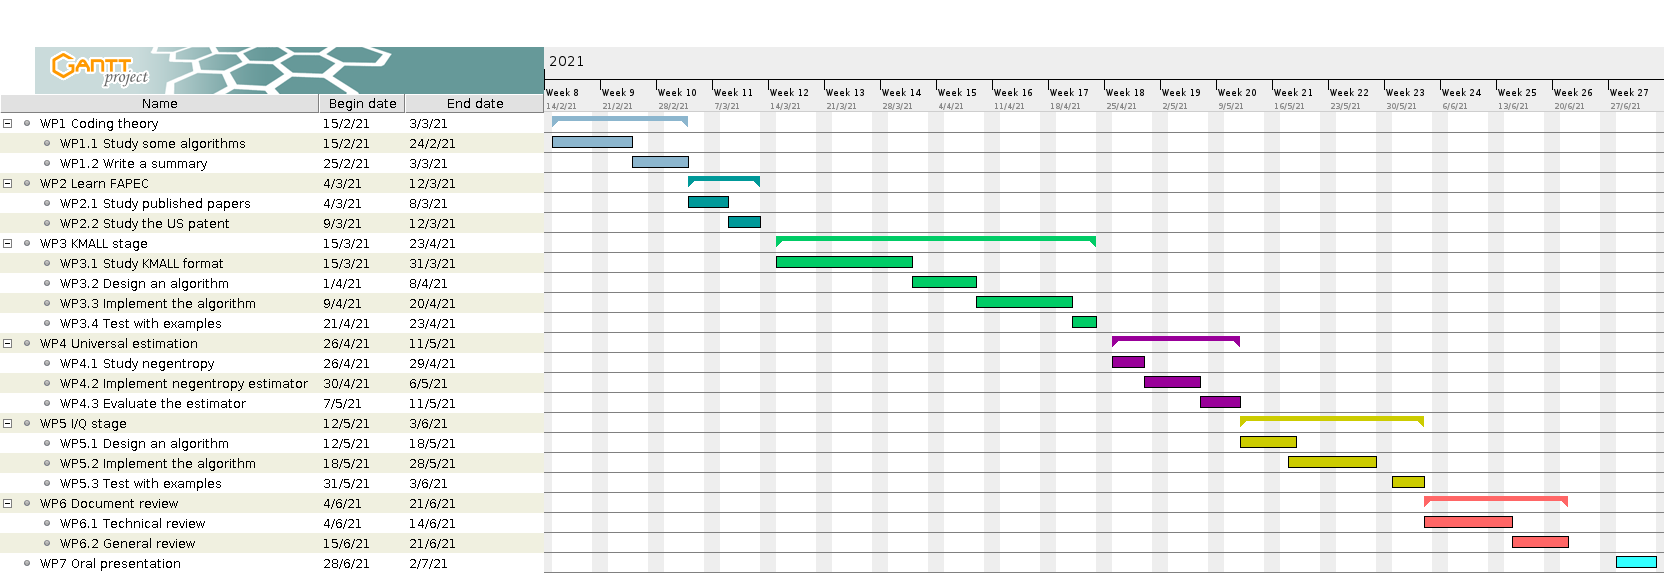
\includegraphics[scale=0.255]{images/gantt.png}
	\end{center}
	\caption{Final Gantt diagram.}
	\label{fig:gantt}
\end{figure}

\subsection{Budget and costs}
This thesis consists in the design, implementation and evaluation of two stages which will be included in a bigger framework, \acrshort{fapec}. In this situation, a straightforward financial study is not possible and going further is clearly out of scope.

However, this thesis has been developed within a cooperation agreement between the Polytechnic University of Catalonia (UPC) and DAPCOM Data Services, with a cost of 3816€.
